%Version 3 December 2023
% See section 11 of the User Manual for version history
%
%%%%%%%%%%%%%%%%%%%%%%%%%%%%%%%%%%%%%%%%%%%%%%%%%%%%%%%%%%%%%%%%%%%%%%
%%                                                                 %%
%% Please do not use \input{...} to include other tex files.       %%
%% Submit your LaTeX manuscript as one .tex document.              %%
%%                                                                 %%
%% All additional figures and files should be attached             %%
%% separately and not embedded in the \TeX\ document itself.       %%
%%                                                                 %%
%%%%%%%%%%%%%%%%%%%%%%%%%%%%%%%%%%%%%%%%%%%%%%%%%%%%%%%%%%%%%%%%%%%%%

%%\documentclass[referee,sn-basic]{sn-jnl}% referee option is meant for double line spacing

%%=======================================================%%
%% to print line numbers in the margin use lineno option %%
%%=======================================================%%

\documentclass[lineno,sn-basic]{sn-jnl}% Basic Springer Nature Reference Style/Chemistry Reference Style

%%======================================================%%
%% to compile with pdflatex/xelatex use pdflatex option %%
%%======================================================%%

%%\documentclass[pdflatex,sn-basic]{sn-jnl}% Basic Springer Nature Reference Style/Chemistry Reference Style


%%Note: the following reference styles support Namedate and Numbered referencing. By default the style follows the most common style.
%%The option is available for: sn-basic.bst, sn-vancouver.bst, sn-chicago.bst%  
 
%%\documentclass[pdflatex,sn-nature]{sn-jnl}% Style for submissions to Nature Portfolio journals
%%\documentclass[pdflatex,sn-basic]{sn-jnl}% Basic Springer Nature Reference Style/Chemistry Reference Style
%%\documentclass[pdflatex,sn-mathphys-num]{sn-jnl}% Math and Physical Sciences Numbered Reference Style 
%%\documentclass[pdflatex,sn-mathphys-ay]{sn-jnl}% Math and Physical Sciences Author Year Reference Style
%%\documentclass[pdflatex,sn-aps]{sn-jnl}% American Physical Society (APS) Reference Style
%%\documentclass[pdflatex,sn-vancouver,Numbered]{sn-jnl}% Vancouver Reference Style
%%\documentclass[pdflatex,sn-apa]{sn-jnl}% APA Reference Style 
%%\documentclass[pdflatex,sn-chicago]{sn-jnl}% Chicago-based Humanities Reference Style

%%%% Standard Packages
%%<additional latex packages if required can be included here>

\usepackage{graphicx}%
\usepackage{multirow}%
\usepackage{amsmath,amssymb,amsfonts}%
\usepackage{amsthm}%
\usepackage{mathrsfs}%
\usepackage[title]{appendix}%
\usepackage{xcolor}%
\usepackage{textcomp}%
\usepackage{manyfoot}%
\usepackage{booktabs}%
\usepackage{algorithm}%
\usepackage{algorithmicx}%
\usepackage{algpseudocode}%
\usepackage{listings}%
\usepackage{float}%
%%%%

%%%%%=============================================================================%%%%
%%%%  Remarks: This template is provided to aid authors with the preparation
%%%%  of original research articles intended for submission to journals published 
%%%%  by Springer Nature. The guidance has been prepared in partnership with 
%%%%  production teams to conform to Springer Nature technical requirements. 
%%%%  Editorial and presentation requirements differ among journal portfolios and 
%%%%  research disciplines. You may find sections in this template are irrelevant 
%%%%  to your work and are empowered to omit any such section if allowed by the 
%%%%  journal you intend to submit to. The submission guidelines and policies 
%%%%  of the journal take precedence. A detailed User Manual is available in the 
%%%%  template package for technical guidance.
%%%%%=============================================================================%%%%

\raggedbottom
%%\unnumbered% uncomment this for unnumbered level heads

\begin{document}

\title[Article Title]{Vegetation structure drives mosquito community composition in UK’s largest managed lowland wetland}

%%=============================================================%%
%% GivenName	-> \fnm{Joergen W.}
%% Particle	-> \spfx{van der} -> surname prefix
%% FamilyName	-> \sur{Ploeg}
%% Suffix	-> \sfx{IV}
%% \author*[1,2]{\fnm{Joergen W.} \spfx{van der} \sur{Ploeg} 
%%  \sfx{IV}}\email{iauthor@gmail.com}
%%=============================================================%%

\author*[1,2]{\fnm{Daniel C} \sur{ Smith}}\email{dansmi@ceh.ac.uk}
\equalcont{These authors contributed equally to this work as first author.}

\author[1]{\fnm{Stefanie M} \sur{Schäfer}}\email{smsc@ceh.ac.uk}
\equalcont{These authors contributed equally to this work as first author.}

%% \author[3]{\fnm{Mick} \sur{Peacey}}\email{Unknown}

%% \author[1]{\fnm{John} \sur{Day}}\email{jcda@ceh.ac.uk}

\author[1]{\fnm{Nick} \sur{Golding}}\email{nick.golding.research@gmail.com}

\author[1]{\fnm{Miles A} \sur{Nunn}}\email{miles.nunn@akaritx.com}

%% \author[3]{\fnm{Rachael} \sur{Madison}}\email{Unknown}

\author[1]{\fnm{Steven M} \sur{White}}\email{smwhit@ceh.ac.uk}

\author[2]{\fnm{Amanda} \sur{Callaghan}}\email{a.callaghan@reading.ac.uk}

\author[1]{\fnm{Bethan V} \sur{Purse}}\email{beth@ceh.ac.uk}


\affil*[1]{\orgdiv{Department}, \orgname{UK Centre for Ecology and Hydrology}, \orgaddress{\street{MacLean Building}, \city{Wallingford}, \postcode{OX10 8BB}, \country{UK}}}

\affil[2]{\orgdiv{School of Biological Sciences}, \orgname{University of Reading}, \orgaddress{\street{Whiteknights}, \city{Reading}, \postcode{RG6 2AJ}, \country{UK}}}

%%\affil[3]{\orgdiv{Department}, \orgname{Organization}, \orgaddress{\street{Street}, \city{City}, \postcode{610101}, \state{State}, \country{Country}}}

%%==================================%%
%% Sample for unstructured abstract %%
%%==================================%%

% \abstract{The abstract serves both as a general introduction to the topic and as a brief, non-technical summary of the main results and their implications. Authors are advised to check the author instructions for the journal they are submitting to for word limits and if structural elements like subheadings, citations, or equations are permitted.}

%%================================%%
%% Sample for structured abstract %%
%%================================%%

\abstract{\textbf{Purpose:} The rising burden of mosquito-borne diseases in Europe extends beyond urban areas, encompassing rural and semi-urban regions near managed and natural wetlands evidenced by recent outbreaks of Usutu and West Nile viruses. While wetland management policies focus on biodiversity and ecosystem services, few studies explore the impact on mosquito vectors. 

\textbf{Methods:} Our research addresses this gap, examining juvenile mosquito and aquatic predator communities in 67 ditch sites within a south England coastal marsh, subjected to different wetland management tiers. Using joint distribution models, we analyse how mosquito communities respond to abiotic and biotic factors influenced by wetland management.

\textbf{Results:} Of the 12 mosquito species identified, \textit{Culiseta annulata} (Usutu virus vector) and \textit{Culex pipiens} (Usutu and West Nile virus vector) constitute 47\% of 6825 larval mosquitoes. Abundant predators include Coleoptera (water beetles) adults, Corixidae (water boatmen), and Zygoptera  (Damselfy) larvae. Models reveal that "Tier 3"   management sites (higher winter water levels, lower agricultural intensity)  associated with shade and less floating vegetation are preferred by specific mosquito species. All mosquito species, except \textit{Anopheles maculipennis s.l.}, are negatively impacted by potential predators. \textit{Culiseta annulata} shows positive associations with shaded and turbid water, contrary to preferences of Corixidae predators.

\textbf{Conclusion:} Tier 3 areas managed for biodiversity, characterised by higher seasonal water levels and reduced livestock grazing intensity, provide favourable habitats for key mosquito species that are known vectors of arboviruses like Usutu and West Nile. Our findings emphasise the impact of biodiversity-focused wetland management, altering mosquito breeding site vegetation to enhance vector suitability. Further exploration of these trade-offs is crucial for comprehending the broader implications of wetland management.}

\keywords{Mosquito, Wetlands, Management, Disease, Community Ecology}

%%\pacs[JEL Classification]{D8, H51}

%%\pacs[MSC Classification]{35A01, 65L10, 65L12, 65L20, 65L70}

\maketitle

\section{Background}\label{sec1}

The burden and risk of mosquito-borne diseases (MBDs) is increasing across Europe, not only in urban areas, driven by invasive Aedes mosquitoes (e.g., Dengue, Chikungunya, Zika, \cite{medlockReviewInvasiveMosquitoes2012}), but also by native species in more rural or peri-urban areas, at the interfaces between human habitation, agriculture, and natural ecosystems (e.g., West Nile virus, Usutu, Sindbis, \cite{buckleySerologicalEvidenceWest2003, chengEvaluatingRiskUsutu2018}). These changes in risk are attributed to multiple interacting global drivers including climate change cite:\citep{bruguerasEnvironmentalDriversClimate2020}, increased trade and travel \citep{benelliAedesAlbopictusAsian2020, kilpatrickGlobalizationLandUse2011}, and land use change, including agricultural intensification and urbanisation \citep{gottdenkerAnthropogenicLandUse2014, meyersteigerMosquitoCommunitiesDisease2016, townroeBritishContainerBreeding2014}. At local scales, altered human behaviour through uptake of activities in areas with long standing mosquito presence can be driver of MBD risk, through increased potential contact time between people and competent vectors \citep{lambinPathogenicLandscapesInteractions2010}. Man-made habitat modification that leads to shifts in abundance and species composition of mosquito populations can also alter the interaction dynamics between mosquitoes, humans, and animal reservoir hosts, increasing the relative risk of zoonotic disease spillover \citep{meyersteigerMosquitoCommunitiesDisease2016}.

In parallel, there is an increased policy focus on managing natural ecosystems such as wetlands to maximise the provision of ecosystem services and enhance biodiversity \cite{acremanTradeoffEcosystemServices2011, defraCountrysideStewardshipGet2023, gibbsWetlandLossBiodiversity2000}. Within the UK, for example, government policies and payment schemes to landowners encourage the creation, restoration, and management of existing wetlands to increase biodiversity and foster local and regional flood resilience programs \citep{defra25YearEnvironment2023, defraCountrysideStewardshipGet2023, defraThirdNationalAdaptation2023a}. Water is a requirement for mosquito breeding and so there is an urgent need to understand how policy-driven changes in wetlands impact mosquito communities, as well as their interactions with animal and human hosts, and how this trades off with disease transmission risk \citep{daleWetlandsMosquitoesReview2008,martinouCallArmsSetting2020,medlockImpactsCreationExpansion2015, hanfordManagementUrbanWetlands2020}. 

There is growing evidence globally that wetland management for biodiversity can affect mosquito communities \citep{reyNorthAmericanWetlands2012}, not only by changing aquatic breeding site characteristics and vegetation but also via impacts on mosquito predators \citep{griffinReviewRoleFish2012, sahaPredationPotentialOdonates2012}, and that this can lead to public health co-benefits or dis-benefits depending on local context. Some studies have found that mosquito density increases after wetland construction and management \citep{schaferBiologicalDiversityRisk2004, jianninoEvaluationVegetationManagement2004}, but if implemented correctly, wetland management schemes that create diverse and permanent wetland habitats can decrease mosquito populations by simultaneously decreasing habitats suitable for larval mosquitoes while increasing those suitable for known mosquito predators \citep{james-pirriEffectsOpenMarsh2009, rochlinIntegratedMarshManagement2012a, rosePesticidesPublicHealth2001a}. Dynamically altering wetland water levels during the mosquito breeding seasons, including complete drying of water bodies during peak breeding months can lead to desiccation of mosquito larvae and prove an adequate control method,  but  these strategies can negatively impact other aquatic flora and fauna of the wetland \citep{russellConstructedWetlandsMosquitoes1999a}. In Australia, draining and re-filling of urban wetlands to manage an invasive fish species, led to increased abundance of mosquito species compared to undrained urban wetlands \citep{hanfordManagementUrbanWetlands2020}. In some contexts, integrated management for biodiversity and reduced public health risks and nuisance biting from mosquitoes has been possible. Aptly named Integrated Marsh Management Schemes employed in salt marshes in the USA, combine tidal flow restoration and vegetation management favouring fish and wildlife biodiversity, with management of open water surfaces (Open Marsh Water Management) to enhance habitats for larvivorous fish predators \citep{rochlinEffectsIntegratedMarsh2012}.


In Europe  and the UK, there is a notable dearth of data regarding the influence of wetland management on mosquito communities, encompassing both nuisance biters and potential disease vectors  \citep{hawkesWetlandMosquitoSurvey2020}. Existing research is limited in its examination of the potential trade-offs between conservation-oriented management practices aimed at preserving biodiversity and their implications for public, animal, and wildlife health \citep{martinouCallArmsSetting2020}. This knowledge gap is increasingly pressing for Europe, particularly considering the reported 3,500 human cases of West Nile fever, resulting in 379 deaths, between 2010 and 2018. Furthermore, the heightened circulation of the Usutu virus, associated with mosquitoes in and around wetlands, adds urgency to the need for a comprehensive understanding of the impacts of wetland management on mosquito communities \citep{ferragutiEffectsLandscapeAnthropization2016}. Specifically, in Southern England, where Usutu virus is currently impacting blackbird populations \citep{follyEvidenceOverwinteringAutochthonous2022a}, and given the proximity to West Nile virus circulation in Germany and the Netherlands \citep{bakonyiWestNileVirus2020}, there is an increased likelihood of further incursions of mosquito-borne pathogens in the short to medium term. Studies conducted in UK fenlands have explored the links between wetland management and mosquito abundance, and revealed that emergent vegetation and sediment build-up can lead to warmer waters and increased densities of Culicine mosquito species, while drainage of water levels can decrease Culicine abundance but create a more suitable habitat for \textit{Anopheles maculipennis s.l.}, a species complex known for its nuisance biting behaviour \citep{medlockSeasonalDynamicsHabitat2015a}.

Combining empirical mosquito surveys with statistical spatial modelling of abiotic and biotic drivers of mosquito  community composition across wetland management gradients may lead to a more detailed understanding of impacts of wetland management on candidate vector species and biting risks. Utilising such an approach in marshes in the east of England (North Kent Marshes), \cite{goldingIdentifyingBioticInteractions2015a} found that ditch shrimp (\textit{Palaemon varians}) and fish predators reduced the prevalence of mosquito larvae, namely of \textit{An. maculipennis s.l.} (a species complex thought to include minor and historical malaria vectors) and \textit{Culex modestus} (a bridge vector for WNV) and suggested that habitat management for these species could both increase biodiversity and reduce mosquito numbers. 

Species distribution models have been applied at national, sub-national and local scales to study the impacts of wetland changes on individual mosquito vector species, but these ignore important species community interactions. However, community modelling approaches such as joint species distribution models \citep{goldingBayesCommBayesianCommunity2015, ovaskainenHowMakeMore2017, pichlerNewJointSpecies2021} might offer great advantages. These models can help identify shared responses to environmental conditions \citep{poggiatoInterpretationsJointModeling2021} and account for potential biotic interactions such as competition and predation. These interactions can strongly influence mosquito population dynamics and persistence \citep{beketovPredationRiskPerception2007a, braksInterspecificCompetitionTwo2004, sahaPredationPotentialOdonates2012} and will likely modulate individual vector species responses to wetland changes \citep{reyNorthAmericanWetlands2012}. 
This study applies community joint modelling methods to sampled larval and adult mosquito population data in a UK wetland that has been subject to management changes under agri-environmental schemes, where water levels, livestock grazing pressure and mechanical interventions are differentially managed, with the following objectives: 

\begin{enumerate}
    \item To understand the role of abiotic (physico-chemical water parameters, ditch morphology, vegetation structure) and biotic factors (predator communities) in determining larval mosquito community composition
    \item To determine whether wetland management changes under recent agri-environmental schemes are likely to have increased the larval abundance and diversity of key UK mosquito vectors of important mosquito-borne viruses.
\end{enumerate}

\section{Methods}\label{sec2}

\subsection{Study site}\label{subsec-study}

The Somerset Levels and Moors (SLM), the largest remaining lowland wet grassland in the UK, spanning 650 km2 in the southwest of England, holds unique ecological significance. Designated under the European Commission Habitats Directive and the UK Biodiversity Action Plan, it serves as an exemplary coastal grazing marsh habitat (JNCC, 1994). This area plays a crucial role in providing essential ecosystem services to local communities and tourists, boasting high biodiversity with a notable presence of wading and migratory birds year-round \citep{acremanTradeoffEcosystemServices2011}.

The SLM's history is marked by periodic winter inundation over the past 10,000 years, contributing to the development of fertile peat soils and rich biodiversity. However, human activities, such as drainage and ditching for seasonal grazing pastures, began as early as the 9th century and intensified in the mid-20th century, reaching a peak with peat extraction and agricultural practices. Recognizing its environmental sensitivity, the SLM received designation as an Environmentally Sensitive Area (ESA) in 1987. Subsequently, agri-environmental schemes were implemented to support farmers in adopting management practices beneficial to biodiversity and flood management \citep{morrisEconomicDimensionsIntegrating2008}. This led to the transformation of arable land back into wet grassland.

Operating in a tiered system, these agri-environment schemes prescribe different measures, including encouraging lower grazing pressure, minimizing mechanical intervention in fields and surrounding ditches, and maintaining higher minimum water levels, especially in winter (Tier 3 versus Tiers 1 and 2). We anticipate that these tiered prescriptions will influence shading, vegetation structure, ditch morphology, and the presence of macro-invertebrate predators. Consequently, these conditions are expected to impact mosquito species. Our study aims to sample and investigate the key drivers of mosquito community composition in Tier 3 versus Tier 1 sites across the SLM, shedding light on the ecological dynamics influenced by wetland management practices.

\subsection{Ecological Survey}\label{subsec2}

We randomly selected 17 ditch locations across two management regimes, eight in Tier 1 management and 9 in Tier 3 of the SLM (Fig 1). At each site, we selected four sampling sites (ditches) within a 500m radius of the location, often part of an interconnected ditch system. We surveyed these sampling sites using a standard dipping protocol across three time points: spring (May), summer (June/July) and autumn (August/September) for three years, from 2009 to 2011. We set up six dip-points, for which we took GPS locations, at each sampling site along the ditch from one to six meters, randomly determined by the throw of a dice.  During each visit, we took a complete submersion dip sample from both water-body margins as well as the centre of the ditch using a 1-liter volume mosquito dipper at each of the dip points. 

We recorded the abundance of mosquito larvae and pupae, and that of potential mosquito predator groups at each dip point. Aquatic macroinvertebrate species were identified in situ to order and suborder, where possible, using \citep{dobsonGuideFreshwaterInvertebrates2012}. Mosquito larvae and pupae were preserved in 70\% ethanol and identified to species or species complex level in the laboratory using the morphological keys by \citep{beckerMosquitoesTheirControl2010b, schaffnerMosquitoesEuropeIdentification2001, cranstonKeysAdultsMale1987a, snowMosquitoes1990a}. During each visit, details of bankside, emergent and floating channel vegetation were recorded \citep{copeGrassesBritishIsles2009a, jermySedgesBritishIsles1995}. Plants within and at the edges of the ditch were identified to genus or species level, and their percentage cover and height estimated. Vegetation height and percentage cover values were averaged across species in three groups based on their functional impact, bank, emergent, and floating vegetation, since these vegetation structures are likely to have differential impacts on habitat suitability across mosquito species (Table \ref{tab:vegetation}). We measured the physicochemical characteristics of the ditch at each sampling site, assessing ditch width, and area of the ditch shaded (a proxy for habitat openness) as well as pH, temperature, turbidity, and salinity of the water. Average values for the covariates listed in Table \ref{tab:vegetation} were summarised across the six dip-points per ditch site in each season.

\begin{sidewaystable}
%% \begin{table}[ht]
\centering
\caption{Effect of Environmental Variables on Mosquito Abundance: Impact and expected ecological implications of key environmental factors on mosquito populations, including vegetation cover, water characteristics, and habitat structure.}
%% \begin{tabular}{p{3cm}p{6cm}p{7cm}}
\begin{tabular}{p{3cm}p{6cm}p{7cm}}
\toprule
\textbf{Variable} & \textbf{Description} & \textbf{Impact on Mosquito Abundance} \\
\midrule
Floating Vegetation Cover (\%) & The percentage of the water surface covered by floating plants or plants with significant leaf coverage. & Expected negative impact on mosquito population density. Dense floating aquatic plants, like \textit{Lemna spp.}, can inhibit mosquito larvae and pupae reaching the water surface for air \cite{cuthbertAquaticPlantExtracts2020, eidEffectDuckweedLemna1992}. \\
\addlinespace
Bank Vegetation Height (cm) & The height of vegetation along the ditch margins and banks. & Increased structural complexity may provide favorable microhabitats for adult mosquitoes and increase availability of sheltered resting places \cite{sauerHabitatMicroclimateAffect2021}. \\
\addlinespace
Bank Vegetation Cover (\%) & The percentage of banks covered by plant matter. & Cover would be expected to provide similar benefits as height.\\
\addlinespace
Emergent Vegetation Height (cm) & The height of vegetation emerging vertically from the waterbody. & Emergent vegetation may provide increased shelter for mosquito females ovipositing on the water surface and improve larval and pupal survival through predator avoidance \cite{sahaHabitatComplexityReduces2009}. \\
\addlinespace
Emergent Vegetation Cover (\%) & The percentage area of emergent vegetation. & Cover would be expected to provide similar benefits as height.\\
\addlinespace
Shaded Water (\%) & Percentage of water surface shaded. & Expected positive impact on mosquito species with a preference for heavily vegetated or cool breeding sites \cite{hawkesWetlandMosquitoSurvey2020}. \\
\addlinespace
Width (cm) & Width of the waterbody. & Wider waterbodies may be more favorable for vertebrate predators, negatively impacting mosquito density \cite{sunaharaHabitatSizeFactor2002}. Some species, like \textit{An. maculipennis s.l.}, prefer more open habitats \cite{hawkesWetlandMosquitoSurvey2020}. \\
\addlinespace
Water Temp (°C) & Water temperature at sampling. & Larval development time is shorter, and survival is better at moderately higher temperatures \cite{bayohTemperatureRelatedDuration2004, meretaPhysicochemicalBiologicalCharacterization2013a, rydzaniczSpeciesCompositionSeasonal2003}. \\
\addlinespace
Dissolved O\textsubscript{2} (ppm) & Concentration of dissolved oxygen in the water. & Uncertain impact as many UK species are tolerant to a broad range of dissolved oxygen levels. \\
\addlinespace
pH & Water acidity/basicity at sampling. & Most mosquitoes prefer neutral pH levels for optimum growth and are tolerant to moderate fluctuations \cite{emidiEffectPhysicochemicalParameters2017}. \\
\addlinespace
Turbidity & Water clarity, indication of water flow. & Turbid waters are expected to increase mosquito larvae survival since predator efficiency is reduced \cite{cano-rocabayeraMosquitoLarvaeConsumption2020, utne-palmVisualFeedingFish2002}. \\
\addlinespace
Salinity (ppt) & Salt content of the water body. & Salinity directly affects mosquito immature presence, with tolerance varying across species \cite{medlockReviewInvasiveMosquitoes2012}. \\
\bottomrule
\end{tabular}
\label{tab:vegetation}
%% \end{table}
\end{sidewaystable}

\begin{figure}[h!htbp]
	\centering
	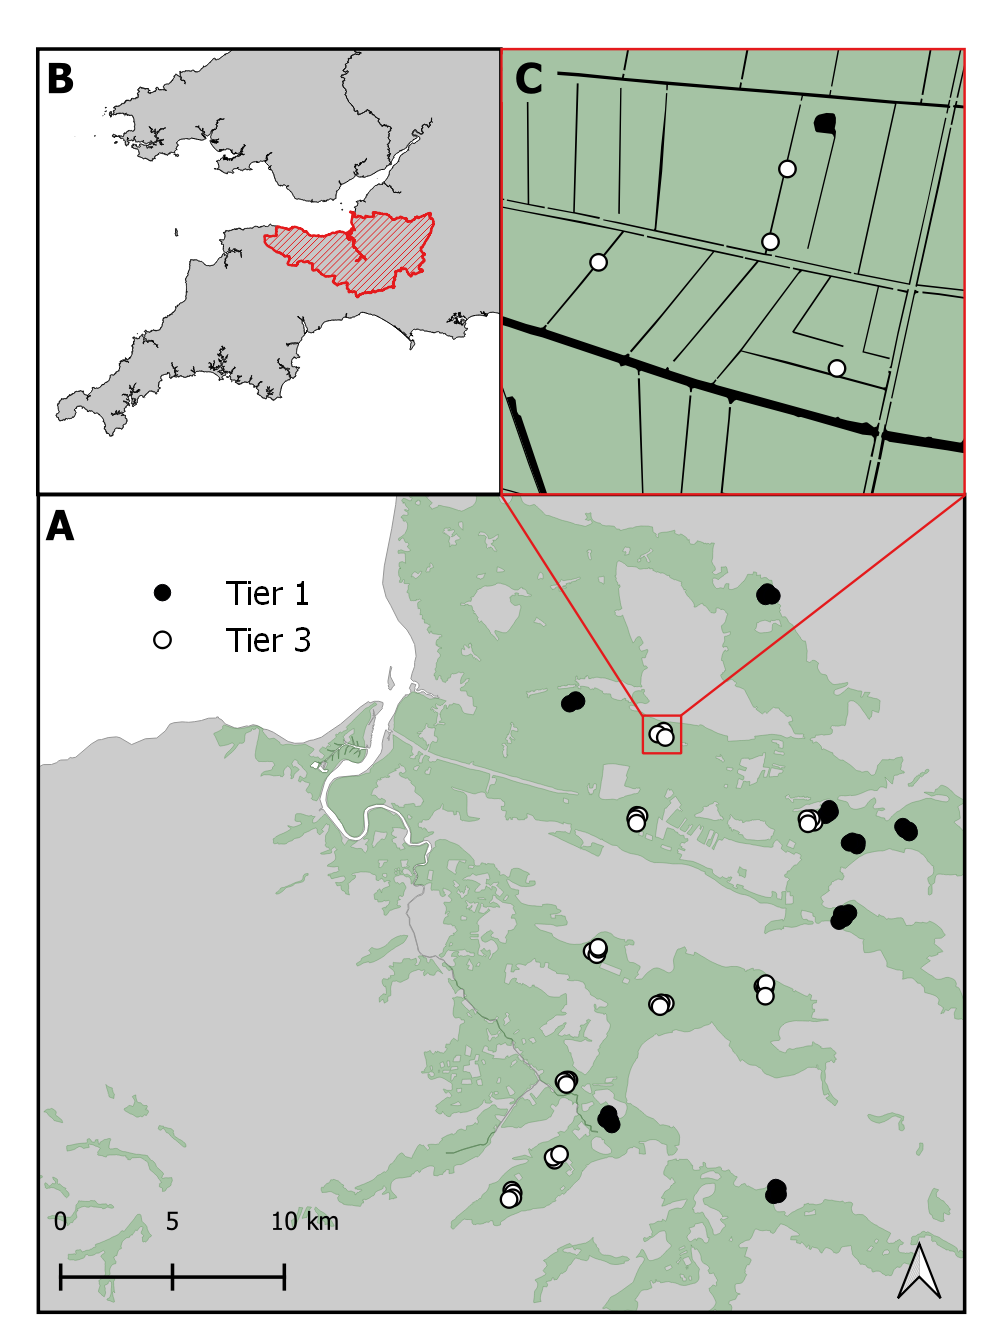
\includegraphics[width=0.9\linewidth]{map}
	\caption{\textbf{A} Map of Somerset Levels and Moors study site. Extent of coastal grazing marsh in green with Tier 1 and Tier 3 locations with sampling sites superimposed (black and white circles respectively). \textbf{B} Location of the study site (red hatching) in South England. \textbf{C} Inset frame showing detailed hierarchical spatial sampling design for each sampling site (circles) in which four ditches were sampled within a 500m square radius for each location.}
	\label{fig:map}
\end{figure}

\subsection{Statistical Analysis}\label{statisticalanalyses}

We used a joint multivariate hierarchical generalized mixed linear model approach, to account for the interdependency of species responses to the environment and species responses to each other in the ecosystem, by modelling all species simultaneously and accounting for each species responses to measured and unmeasured environmental covariates through latent variable factors \citep{wilkinsonComparisonJointSpecies2019}. We fitted our model using the R package Hierarchical Modelling of Species Communities (HMSC; \cite{ovaskainenHowMakeMore2017, ovaskainenJointSpeciesDistribution2020}) framework, to explore how biotic and abiotic interactions drive mosquito larval distribution across the SLM. 

The multispecies generalised linear latent variable model (with probit link function) was fitted to the presence-absence data for 4 mosquitoes and 8 predator groups obtained from our 320 sampling sites with abiotic covariates on a linear scale (Table \ref{tab:vegetation}). We excluded any species that occurred fewer than ten times to increase statistical stability \citep{ovaskainenJointSpeciesDistribution2020}, leading to the exclusion of one mosquito species and four predator groups (see results). To account for potential spatial biases in the sampling data, we generated a distance matrix, calculated from the average coordinates across the six dip points that make up each sampling site, to represent the spatial scales between each sampling unit as a spatially structured random effect \citep{f.dormannMethodsAccountSpatial2007}. We considered the impact of temporal effects on sampling methods by including a nested random effect for both year and time point. In this case we consider the height and areal cover of different plant functional groups bank, emergent, and floating vegetation) as an abiotic driver as we expect them to function as a regulator of population fitness through shielding of predation or similar processes \citep{sahaHabitatComplexityReduces2009}.

The model was fitted using four Monte-Carlo Markov Chains (MCMC) with a transient period of 5000 samples and target of 1000 samples per chain using a thinning rate of 1000 for a total of 4 million MCMC post-transient in samples in total. Parameter convergence was measured using Gelman and Rubens potential scale reduction factor (PSRF, \cite{gelmanInferenceIterativeSimulation1992}). We used five-fold cross validation to validate model performance, comparing predictive and explanatory values of Tjur’s R2 and the area under curve (AUC) statistic for each species \citep{loboAUCMisleadingMeasure2008, tjurCoefficientsDeterminationLogistic2009}. We examined the importance of different sets of covariates in our model by partitioning the variation explained by fitting of partial models \citep{borcardPartiallingOutSpatial1992, ovaskainenJointSpeciesDistribution2020}. We originally aimed to construct abundance models that included the same covariates, as we hypothesised that biotic interactions would have a greater impact on species abundance than species presence. However, due to the high complexity of the model, it was deemed computationally infeasible to achieve an acceptable fit and run-times exceeded one month without reasonable convergence for all species \citep{howardImprovingSpeciesDistribution2014}.

To understand if management tiers influence potential abiotic drivers of mosquito populations, we estimated the marginal effect of management tier on each covariate measured in our sampling procedure (Table \ref{tab:vegetation}). We modelled each covariate separately against management level as a categorical factor, with both a random effect for site and a nested random effect of season within year to account for temporal differences in covariate distribution. Bayesian multivariate models were built in the probabilistic programming language Stan using the BRMS package in R \citep{carpenterStanProbabilisticProgramming2017, burknerBrmsPackageBayesian2017}. Covariates measured on a percentage scale (metrics of vegetation cover and shaded area) used a Zero-One Inflated Beta response distribution. Bank and emergent vegetation height used lognormal hurdle mixed response distributions to account for over-dispersion and the influence of zero values. All other covariates used a student-t distribution for robust estimation of parameter values. Significance was measured across the 95\% CI using mean equal tailed intervals of the posterior distribution. 

\section{Results}\label{results}

\subsection{Differences in environmental conditions between management tiers}
Metrics of ditch vegetation structure differed significantly between sites subject to Tier 1 versus Tier 3 management, whilst physicochemical properties of the waterbody and ditch structure parameters did not (Table \ref{tab:tier-model}, \textbf{Table S1}). Though water-bodies were on average 8cm wider in Tier 3 managed areas, this difference was not statistically significant (95\% CI [-23.94, 6.31]). There was no measurable difference in turbidity (95\% CI [-0.15, 0.18]) or salinity (95\% CI [-0.12, 0.15]) between the management tiers, and pH values were on average -0.3 lower in Tier 3 areas, but this was also non-significant (95\% CI [0.03, 0.65]). 

Bank vegetation was more likely to be present (95\% CI [-0.29, -0.10], Table S1), and when present it was significantly taller, by 25cm on average (95\% CI[-55.78, -4.24]), in Tier 3 ditches than Tier 1 ditches, but we found no differences in the levels of bank-side vegetation cover between tiers (Mean = 0.01, 95\% CI[-0.05,0.07]) . Similarly, we found that emergent channel vegetation was 29\% more likely to be present in Tier 3 areas (95\% CI [-0.39, -0.18]), and when emergent vegetation was present it was 5cm taller on average than in Tier 3 areas than Tier 1 areas (95\% CI [-12.39, -0.34]). There was no measurable difference in the probability of floating vegetation cover being 0\% (95\% CI[-0.15, 0.06]) or 100\% (95\% CI[-0.1, 0.04]) between tiers, but on average there was 10\% less floating vegetation cover in Tier 3 areas than in Tier 1 areas and this was significant (95\% CI[0.01, 0.19]). The amount of shaded area of the channel did not vary significantly between tiers (Mean = 0.12 95\% CI[-0.01, 0.27]), but the probability of a waterbody being completely shaded was 48\% higher in Tier 3 areas than Tier 1 (95\% CI[-0.8, -0.2]), and the probability of a waterbody having no shade was 10\% more likely in Tier 3 areas (95\% CI[0.03, 0.016]). 

\begin{sidewaystable}[htbp]
	\centering
	\caption{Differences in environmental variables between the Tier 1 (T1) and Tier 3 (T3) wetland management regimes. Table shows the marginal effect of Management Tier for each environmental covariate from pairwise posterior distribution contrasts of T1-T3 values. PD (Probability of Direction) estimates above 97.5 are deemed significant and highlighted in bold. MPE (Mean Parameter Estimates) with Lower MPE$_{Low}$ and Upper MPE$_{High}$ estimates represent the equal tailed 95\% CI estimate across the model’s posterior distribution. Full parameter estimates for each model covariate are given in Table S1.}\label{tab:tier-model}
	\begin{tabular}{l l c c c c}
		\toprule
		\textbf{Model Covariate} & \textbf{Effect of Tier 3} & \textbf{PD (\%)} & \textbf{MPE} & \textbf{MPE$_{low}$} & \textbf{MPE$_{High}$} \\
		\midrule
		Salinity & -- & 57.40 & 0.01 & -0.12 & 0.15 \\
		Emergent Vegetation Height (Height$ _{Emerg} $) & Taller Emergent Vegetation & 98.41 & -5.30 & -12.39 & -0.34 \\
		Dissolved Oxygen (DO$ ^{2} $) & -- & 89.17 & 6.59 & -4.10 & 17.40 \\
		pH & -- & 96.53 & 0.30 & -0.03 & 0.65 \\
		Turbidity & -- & 59.00 & 0.02 & -0.15 & 0.18 \\
		Floating Vegetation Cover (Cover$ _{Float} $) & Less Floating Vegetation Cover & 98.33 & 0.09 & 0.01 & 0.19 \\
		Bankside Vegetation Cover (Cover$ _{Bank} $) & -- & 76.62 & 0.01 & -0.05 & 0.07 \\
		Emergent Vegetation Cover (Cover$ _{Emerg} $) & -- & 70.88 & -0.01 & -0.04 & 0.02 \\
		Water Temperature & -- & 88.33 & -0.82 & -2.24 & 0.59 \\
		Shaded & -- & 96.37 & 0.12 & -0.01 & 0.27 \\
		Ditch Width & -- & 87.67 & -8.58 & -23.94 & 6.31 \\
		Bank Vegetation Height (Height$ _{Bank} $) & Taller Bank Vegetation & 99.62 & -25.28 & -55.78 & -4.24 \\
		\bottomrule
	\end{tabular}
\end{sidewaystable}


\subsection{Abundance and prevalence of sample mosquito and predator taxa}
We recorded twelve different aquatic macroinvertebrates taxa in the SLM of which five were mosquitoes (Table \ref{tab:abundance}). We identified 6896 mosquito larvae in total. \textit{Culiseta annulata} (n = 3250, 47.13\%) and \textit{Culex pipiens} (n = 3248, 47.10\%) made up the highest proportion of these larvae, followed by \textit{Anopheles claviger} (n = 292, 4.23\%) and \textit{Anopheles maculipennis} s.l. (n = 105, 1.52\%). \textit{Anopheles maculipennis s.l.} were most prevalent, occurring in 13\% of the sample sites, followed by \textit{Cs. annulata} (12\%), \textit{An. claviger} (11\%), \textit{Cx. pipiens} (10\%), and lastly \textit{Aedes (Ochlerotatus) caspius} which was present in just a single sampling site (> 0.1\%). Because of the low abundance and low prevalence, \textit{Ae. caspius} was omitted from the subsequent analysis.

We identified eight potential predator taxa that were prevalent across at least 10 sites to be included in this statistical analysis (Table \ref{tab:abundance}). Of these taxa, adult \textit{Coleoptera} (water beetles) were most prevalent, being present in the most sampling units (27\%, n = 308) predator individuals recorded), followed by Corixidae (water boatmen) which were also the most abundant predator species (26\%, n = 647), Zygoptera larvae (damselflies, 25\%, n = 349) and Coleoptera larvae (19\%, n = 139). The other four taxa had a much lower prevalence and abundance across all sampling units, including Gammaridae (\textit{Palaemon varians} or common ditch shrimp, 8\%, n = 103), Anisoptera larvae (dragonflies, 5\%, n = 31), \textit{Ilyocoris cimicoides} (Saucer bugs, 3\%, n = 19) and \textit{Nepa cinerea} (Water scorpions, 3\%, n = 11).

\begin{table}[htbp]
\centering
\caption{Relative prevalence (rate of occurrence across all sites) and total (and proportional) abundance of mosquito and predator taxa across sampled sites among sampled individuals across study sites.} \label{tab:abundance}
\begin{tabular}{lccc}
\toprule
\textbf{Taxon} & \textbf{Prevalence (\%)} & \textbf{Abundance (Total)} & \textbf{Mean Abundance per Sample Site} \\
\midrule
\textit{Anopheles maculipennis} & 13 & 105 & 2.44 $\pm$ 2.22 \\
\textit{Anopheles claviger} & 11 & 292 & 8.11 $\pm$ 11.84 \\
\textit{Culex pipiens} & 10 & 3248 & 101.50 $\pm$ 244.43 \\
\textit{Culiseta annulata} & 13 & 3250 & 81.25 $\pm$ 160.62 \\
Corixidae & 26 & 647 & 7.70 $\pm$ 20.89 \\
Coleoptera larvae & 19 & 139 & 2.24 $\pm$ 1.70 \\
Coleoptera adults & 27 & 308 & 3.58 $\pm$ 3.30 \\
Zygoptera larvae & 26 & 349 & 4.20 $\pm$ 5.55 \\
Anisoptera larvae & 5 & 31 & 1.82 $\pm$ 1.42 \\
\textit{Ilyocoris cimicoides} & 3 & 19 & 1.90 $\pm$ 2.18 \\
\textit{Nepa cinerea} & 3 & 11 & 1.10 $\pm$ 0.32 \\
Gammaridae & 8 & 103 & 4.29 $\pm$ 4.65 \\
\bottomrule
\end{tabular}
\end{table}

\subsection{Overall accuracy of community models and partitioning of variance between key sets of drivers}
Parameter convergence of the HMSC model was satisfactory with all chains generating sufficient effective samples and PSRF values (\textbf{Fig S2}). Explanatory AUC values (for the training dataset) were high for all mosquito species (0.86-0.99) and predictive AUC values (from the cross-validation) were reasonable (0.75-0.89). Explanatory AUC values were similarly high for potential predator taxa, but predictive AUC values were much lower for some of the less abundant taxa (\textit{Nepa cinerea} = 0.4, \textit{Ilyocoris cimicoides}= 0.55, \textit{Anisoptera} larvae = 0.55, \textit{Coleoptera }larvae = 0.57). All other predator taxa had adequate predictive AUC values above 0.69 (Table \ref{tab:accuracy}). 

Metrics of variance explained for the training dataset were higher for Culicine species (\textit{Cx. pipiens s.l.} Tjur’s R$ ^{2} $ = 0.47 ; \textit{Cs}. \textit{annulata} Tjur’s R$ ^{2} $ = 0.55 ) than Anopheline species (\textit{An}. \textit{maculipennis} s.l. Tjur’s R$ ^{2} $ = 0.12; \textit{An}. \textit{claviger} (Tjur’s R$ ^{2} $ = 0.23). When examining the importance of different sets of covariates, for mosquito species, we found that spatiotemporal effects accounted for on average 43\% (SD 29\%) of all variation explained by the models (Fig \ref{fig:variance}, \textbf{Table S3}). Tjur’s R$ ^{2} $ values for predator taxa were much lower than for the mosquito species, except for Corixidae (Tjur’s R$ ^{2} $ = 0.27) and Zygoptera (Tjur’s R$ ^{2} $ = 0.28) larvae. 

Random effects accounted for substantial variation in Culicine species and low amounts of variation for Anopheline species (Fig \ref{fig:variance}). For the Anopheline species, a higher proportion of variance was explained by chemical and channel structure covariates than for Culicine species. Temporal effects of year and season explained less variation in presence of mosquito species compared to the predator taxa, and little in Anopheline species (\textbf{Table S3})

\begin{table}[htbp]
    \centering
    \caption{Accuracy with which community models explained and predicted the distributions of mosquito and predator taxa including Under the Curve (AUC) and Tjur's R\textsuperscript{2} values for explanation and prediction.} \label{tab:accuracy}
    \begin{tabular}{lcccccccc}
        \toprule
        \textbf{Taxa} & \textbf{Explanatory} & & \textbf{Predictive}  \\
        \cmidrule(lr){2-5}
        &  \textbf{AUC} & \textbf{R\textsuperscript{2}} & \textbf{AUC} & \textbf{R\textsuperscript{2}} \\
        \midrule
        \textit{Anopheles maculipennis s.l.} & 0.86 & 0.12 & 0.75 & 0.06 \\
        \textit{Anopheles claviger} & 0.91 & 0.23 & 0.84 & 0.14 \\
        \textit{Culex pipiens} s.l. & 0.98 & 0.40 & 0.84 & 0.22 \\
        \textit{Culiseta annulata} & 0.99 & 0.53 & 0.89 & 0.38 \\
        Corixidae & 0.88 & 0.27 & 0.82 & 0.21 \\
        Coleoptera larvae & 0.78 & 0.08 & 0.57 & 0.02 \\
        Coleoptera & 0.81 & 0.15 & 0.69 & 0.08 \\
        Zygoptera larvae & 0.89 & 0.27 & 0.80 & 0.19 \\
        Anisoptera larvae & 0.86 & 0.03 & 0.55 & 0.00 \\
        \textit{Ilyocoris cimicoides} & 0.87 & 0.03 & 0.50 & 0.00 \\
        \textit{Nepa cinerea} & 0.99 & 0.04 & 0.40 & -0.01 \\
        Gammaridae & 0.87 & 0.14 & 0.76 & 0.08 \\
        \bottomrule
    \end{tabular}
\end{table}


\begin{figure}[h!htbp]
\centering
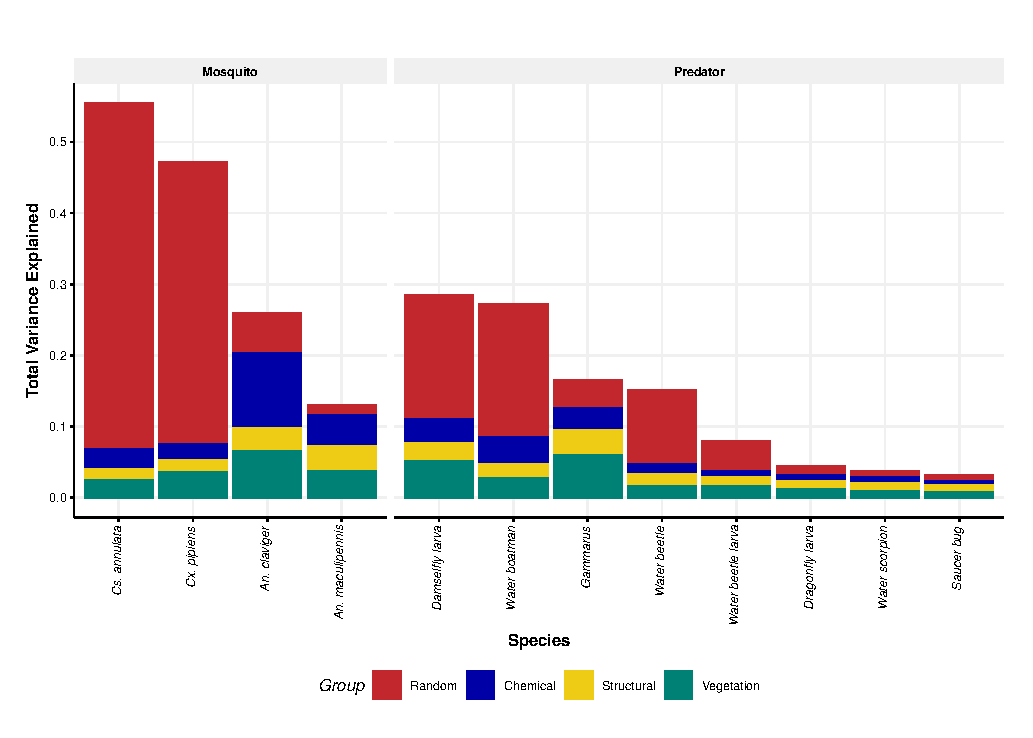
\includegraphics[width=0.9\textwidth]{VP.pdf}
\caption{Variance partitioning and total variance explained by each component for larval mosquitoes and predator species prevalent in the study side. Random effects are the variance explained by year season and the spatial component of the model summed for each species. The “chemical” category includes the physicochemical covariates pH, dissolved oxygen, salinity, turbidity and water temperature, the “structural” category includes the width and relative shadiness of the water body, and the “vegetation” category includes all vegetation metrics; floating, emergent and bank, as covariates in the model. Detailed breakdown of the variance explained by the random effects is provided in Table S3.} \label{fig:variance}
\end{figure}

\subsection{Larval mosquito responses to environmental drivers}

\textit{Culex pipiens} was significantly positively associated with bank vegetation cover (Mean = 0.03, 90\% CI[0.01,0.04]), negatively associated with bank vegetation height (Mean = -0.006, 90\% CI[-0.017,-0.001], and negatively associated with floating vegetation cover (Mean = -0.01 90\% CI[-0.018, -0.001]) (Fig \ref{fig:environment}). \textit{Culiseta annulata} was significantly positively associated with more bankside vegetation cover (Mean = 0.02, 90\% CI[0.001,0.035]) and high turbidity areas (Mean =1.41, 90\% CI[0.28,2.65]). \textit{Anopheles }\textit{maculipennis s.l.} showed strong preference for habitats with little shade (Mean = -1.13, 90\% CI[-2.20,-0.13]) and higher levels of emergent vegetation (Mean = 0.015 90\% CI[0.004,0.026]) (Fig \ref{fig:environment}).\textit{ Anopheles claviger }exhibited a strong preference for shaded habitats (Mean = 1.23, 90\% CI[0.34,2.17]), and ditches with little floating vegetation cover (Mean = -0.015 90\% CI[-0.025,-0.006]) (Fig \ref{fig:environment}).

Several potential predator taxa were also significantly correlated with an array of physicochemical and vegetation drivers (Fig \ref{fig:environment}), but we only interpret these further for those predatory taxa for which a larger percentage of variance in occurrence was explained by the model, namely water boatmen (Corixidae spp) and damselfly larvae (Zygoptera, Fig \ref{fig:variance}). The probability of occurrence of water boatmen was significantly negatively associated with lower shading of waterbodies (Mean = -0.96, 90\% CI[-1,74,-0.23]). The probability of occurrence of damsel fly (Zygoptera spp) larvae was significantly positively impacted by higher levels of floating (Mean = 0.009, 90\% CI[0.003,0.015]) and height of bank vegetation (Mean = 0.005, 90\% CI[0.001,0.009], Fig \ref{fig:environment}).

\begin{figure}[h!htbp]
\centering
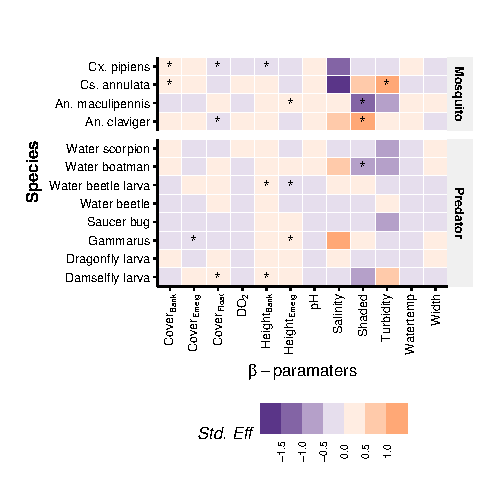
\includegraphics[width=0.9\textwidth]{beta_90.pdf}
\caption{Species responses to covariates by standardised coefficient effect size. “\textbf{*}” Indicates significance of parameter and cells that are blank indicate where the effect was not significant i.e., the 90\% credible interval bridged zero. Height$ _{Emerg} $ = Emergent Vegetation height, Height$ _{Bank} $ = Emergent Vegetation height, Cover$ Float $ = Floating Vegetation cover, Cover$ _{Bank} $ = Bank Vegetation height, Cover$ _{Emerg} $ = Emergent Vegetation cover.}\label{fig:environment}
\end{figure}

\subsection{Residual association between species}

We found significant positive residual species associations between all mosquito species except \textit{An. maculipennis} s.l. after accounting for environmental responses in the HMSC community model (Fig \ref{fig:correlation}). Additionally, we found that all species of mosquito except \textit{An. maculipennis} s.l. show significant negative associations with potential predator taxa including water beetle larvae and adults (Coleoptera), and damselfly (Zygoptera) larvae, water boatmen (Corixidae) and Gammaridae. Saucer bugs (\textit{Ilyocoris)}, dragonfly (Anisoptera) larvae and water scorpions (\textit{Nepa cinerea)} do not show any significant associations with any other species. All other predator taxa show significant positive associations with one another (Fig \ref{fig:correlation}). 

\begin{figure}[h!htbp]
\centering
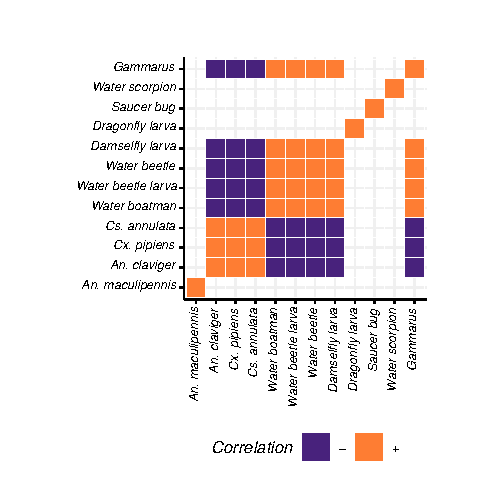
\includegraphics[width=0.9\textwidth]{omega2_90.pdf}
\caption{Significant species residual correlations drawn from the $\Omega$ model parameter for each species in Hmsc. Coloured regions show which species meet the 95\% significance threshold and are expected to be found together more than can be explained by model covariates alone. Correlations that don’t meet this significance threshold are blank. }\label{fig:correlation}
\end{figure}

\section{Discussion}

\subsection{Vegetation structure as a key driver of mosquito communities including potential vectors.}

Increased water levels in Tier 3 areas have been previously shown to favour the establishment of wetland meadow plant species which increase the diversity and quality of vegetation in these areas compared to Tier 1 areas \citep{acremanTradeoffEcosystemServices2011}. Our study supports this, with Tier 3 areas leading to significant increases in emergent and bankside vegetation height, increasing the structural complexity of vegetation compared to Tier 1 areas (Table \ref{tab:tier-model}). 

Areas such as wetlands and marshes tend to harbour a wide variety of mosquito species, due to the presence of a variety of suitable water bodies for oviposition, and aquatic plants that provide shelter, food, and protection from predators, as well as a diverse set of host species from which to draw bloodmeals \citep{medlockPotentialTransmissionWest2005a, beckerMosquitoesTheirControl2010b}. Adult mosquitoes benefit from structural complexity of vegetation, this complexity includes features such as diverse plant species, varied plant heights, and the presence of multiple layers of vegetation, all of which contribute to the creation of sheltered, shaded, and protected spaces. Such complexity in vegetation structure provides suitable conditions for adult mosquitoes, offering refuge from direct sunlight, wind, and other environmental elements, thereby enhancing their overall habitat suitability. that provides shelter, shade and protection from the sun and wind \citep{beckerMosquitoesTheirControl2010b}. Juvenile mosquitoes may also perceive similar benefits from the underwater structures of algae and plant roots as refuges from predators \citep{collinsEffectsRemovalReduction2019a}. A review by \cite{reyNorthAmericanWetlands2012} found that wetlands with high vegetative complexity had a greater diversity of mosquito species compared to wetlands with low vegetative complexity. Consistent with these prior studies, we found that occurrence of three of the key mosquito species in the study area (\textit{An. claviger} and \textit{An. maculipennis s.l.}, and to a lesser extent, the \textit{Cx. pipiens} complex) was favoured by more complex channel vegetation structure characteristic of Tier 3 management (increased height and cover of emergent and bankside vegetation, Table \ref{tab:tier-model}). Consistent with the associations described by \cite{hawkesWetlandMosquitoSurvey2020}. \textit{An. maculipennis} s.l. showed significant preference for less shaded environments suggesting a preference for open style habitats, while \textit{An. claviger} showed a preference for heavily shaded habitats (Fig \ref{fig:environment}). \textit{Cx. pipiens }and\textit{ An. claviger, }both of which can cause significant biting nuisances, are likely to find Tier 3 areas more favourable because of their preference for little floating vegetation (Fig \ref{fig:environment}, Table \ref{tab:tier-model}). Floating vegetation can provide a physical barrier between mosquito and oviposition site as well as larvae and air, dissuading oviposition in these areas \citep{eidEffectDuckweedLemna1992}. Yet, previous studies have found positive associations between floating vegetation cover and mosquito species presence, suggesting the impacts of this factor on mosquito larvae is complex and context-dependent \citep{cuthbertAquaticPlantExtracts2020, goldingIdentifyingBioticInteractions2015a}. 

Except for the association of turbid water with \textit{Cs. annulata} presence, no significant effects of physicochemical characteristics of the water on mosquito occurrence were found (Fig \ref{fig:environment}). This aligns with prior knowledge that Culicine species, \textit{Cx. pipiens }and \textit{Cs. annulata} utilise a breadth of oviposition sites, including drainage ditches, artificial containers, and small stagnant waters, that vary widely in water parameters (Hawkes et al., 2020). We found that physicochemical factors had a larger contribution to variance explained for the Anopheline species. \textit{Anopheles maculipennis s.l.}, and \textit{An. claviger,} at 11\% and 6\% respectively, suggesting more restricted oviposition site preferences. The SLM system is an interconnected network of ditches that covers an area over several hundred square kilometres, leading to relatively homogeneous water chemistry across our study area. This means that the range of conditions experienced by our sampled species might not be large enough to elucidate any meaningful differences in water parameter preferences (and indeed the Tier management regimes did not differ significantly in physico-chemical conditions). 

\subsection{Biotic drivers of larval mosquitoes}

Consistent with prior studies of mosquito community composition at landscape level, we found that biotic interactions may affect the distribution of mosquitos across a wetland environment \citep{goldingIdentifyingBioticInteractions2015a}. Many of the potential predator taxa such as dragonfly and damselfly larvae are frequently observed as effective larval mosquito predators in other contexts and indeed some such as dragonfly larvae have been investigated for biological control of mosquitoes (Medlock and Snow, 2008; Onyeka, 1983; Saha et al., 2012). Water beetles and water boatmen have also been implicated in mosquito larval predation, but their relative predation pressure is thought to be linked to the vulnerability of mosquito larvae \citep{jeffriesIndividualVulnerabilityPredation1988a, medlockNaturalPredatorsParasites2008}. 

As described above, vegetation structure in and around waterbodies affects the availability of refugia from predators and consequently the effectiveness of predator avoidance strategies of immature mosquitoes \citep{sahaHabitatComplexityReduces2009}. Environments with complex underwater vegetation limit the space for predators and mosquito larvae to interact and reduces overall predator efficiency \citep{sahaHabitatComplexityReduces2009, sunaharaHabitatSizeFactor2002}. The higher cover and height of emergent vegetation detected in Tier 3 areas could provide complex vegetation structure both above and below the water level, providing shady refugia that improve predator avoidance in these sites. 

It's crucial to recognise that the species interactions deduced from residual correlations in joint occurrence models are not as dependable as direct observations of predator-prey interactions. Instead, these inferred interactions may be indicative of unmeasured factors such as shared or non-shared environmental preferences between species \citep{poggiatoInterpretationsJointModeling2021}. In essence, while joint occurrence models provide valuable insights, caution should be exercised in attributing the correlations solely to direct predator-prey interactions, as other environmental factors might contribute to the observed patterns \citep{zurellJointSpeciesDistribution2018}. For example, though some mosquito species were found to be negatively correlated with Gammaridae we suspect this may reflect different preferences for unmeasured environmental conditions, since the UK Gammarus species (\textit{Palaemon varians}) is omnivorous and occupies different depths of the waterbodies to mosquito larvae, leading to limited potential predation opportunities (P. Scarlett, \textit{pers comm}, June 2023).

The community models exhibited relatively lower performance for predator species when compared to mosquito species. This implies that to comprehensively grasp how wetland management may influence predator effects on mosquito populations in this context, additional and more detailed data on predators, with improved taxonomic resolution, could be valuable. It's worth considering that while this suggestion is important, it may not be the exclusive solution, and other approaches could also contribute to a more nuanced understanding. Prior studies seem to suggest that management plans targeting biodiversity, such as that seen in Tier 3, will have a positive impact on abundance of key predator taxa such as fish \citep{chandraMosquitoControlLarvivorous2008a, griffinReviewRoleFish2012}. Increased predator abundance would provide a potential control agent for mosquito populations, but few studies have shown this in the field, and none in the UK \citep{griffinReviewRoleFish2012, medlockNaturalPredatorsParasites2008, sahaPredationPotentialOdonates2012}. Our study indicates that water beetle larvae and adults, dragonfly, and damselfly nymphs, and water boatmen may be key predator taxa that play a role in regulating mosquito populations within lowland wet grasslands, and that these roles should be investigated further to fully understand trade-offs between biodiversity management and mosquito biting risk. 

\section{Conclusion}

We have shown here how management schemes directed at increasing the biodiversity of grazed wetlands, could increase the suitability of those habitats for immatures of some key mosquito vectors and nuisance biters, encouraging diverse vegetation structure in and around water bodies, that may reduce their vulnerability to predators. However, thinning or removal of vegetation is not a viable strategy to control mosquito populations, being at odds with the targets of wetland management strategies. Vegetation removal impinges upon important wetland ecosystem functions by decreasing biodiversity, lowering water quality and reducing flood resilience of an area \citep{acremanTradeoffEcosystemServices2011, rochlinEffectsIntegratedMarsh2012}.

Furthermore, to interpret disease risk given future incursions of viruses such as West Nile virus, Sindbis virus or Usutu virus into the UK, it would be necessary to understand how these impacts of wetland management on juvenile mosquito populations cascade through into impacts on the ratio of adult vectors to susceptible hosts (a key parameter in disease transmission \citep{smithRiskMosquitoBorneInfectionin2004a}, by sampling adult vectors, hosts and their interactions (e.g., via blood meal analysis) across wetland gradients into areas of human habitation \citep{hanfordManagementUrbanWetlands2020}. This would provide the evidence-base for co-development of integrated mosquito management and risk awareness strategies among cross-sectoral stakeholders that would minimise risk of exposure while aligning with environmental wetland management goals \citep{martinouCallArmsSetting2020}. Given the diverse and growing mosquito-borne pathogen threats to people living in and around wetland ecosystems, and the diverse assemblages of potential mosquito vector species involved, the combination of joint models with empirical surveys provides an effective way of inferring the complex ecological interactions that will underpin the trade-offs between disease risk and wetland management.

\backmatter

\bmhead{Supplementary information}

Supplementary info contained within S1.docx. This contains Figure S1 and Table S2.

%% \bmhead{Acknowledgements}


\section*{Declarations}

\subsection{Funding}
This research was supported by the QMEE CDT, funded by NERC grant number NE/P012345/1. Additional support was provided to BP, SMS, MN, NG from the Natural Environment Research Council National Capability allocation to UKCEH ( HARM project, EMMPOWER project).
\subsection{Conflicts of Interest}
The authors report no conflicts of interest or competing interests.
\subsection{Eithcs approval and consent}
Not applicable.
\subsection{Consent for publication}
Not applicable.
\subsection{Data availability}
Data are available on GitHub/Dryad (https://github.com/dansmi-hub/Smith2023/tree/master) \textbf{\textit{To be committed to the repository shortly and archived when accepted}}
\subsection{Materials availability}
Not applicable.
\subsection{Code availability}
Reproducible code is available on GitHub (https://github.com/dansmi-hub/Smith2023/tree/master)
\subsection{Author contribution}
The study was conceived by Daniel Smith, Stefanie Schäfer, Bethan Purse, and Miles Nunn. Field data collection and processing were carried out by Stefanie Schäfer, Miles Nunn, Bethan Purse, Nick Golding. Daniel Smith and Bethan Purse performed modelling and statistical analyses. Daniel Smith, Stefanie Schäfer, and Bethan Purse all contributed in writing the manuscript. The manuscript received valuable feedback and comments from Amanda Callaghan and Steven White.

%% \begin{appendices}

%% \section{Section title of first appendix}\label{secA1}

%%An appendix contains supplementary information that is not an essential part of the text itself but which may be helpful in providing a more comprehensive understanding of the research problem or it is information that is too cumbersome to be included in the body of the paper.

%%=============================================%%
%% For submissions to Nature Portfolio Journals %%
%% please use the heading ``Extended Data''.   %%
%%=============================================%%

%%=============================================================%%
%% Sample for another appendix section			       %%
%%=============================================================%%

%% \section{Example of another appendix section}\label{secA2}%
%% Appendices may be used for helpful, supporting or essential material that would otherwise 
%% clutter, break up or be distracting to the text. Appendices can consist of sections, figures, 
%% tables and equations etc.

%% \end{appendices}

%%===========================================================================================%%
%% If you are submitting to one of the Nature Portfolio journals, using the eJP submission   %%
%% system, please include the references within the manuscript file itself. You may do this  %%
%% by copying the reference list from your .bbl file, paste it into the main manuscript .tex %%
%% file, and delete the associated \verb+\bibliography+ commands.                            %%
%%===========================================================================================%%

\bibliography{Smith_2024.bib}% common bib file
%% if required, the content of .bbl file can be included here once bbl is generated
%%\input sn-article.bbl


\end{document}
